\documentclass{article}
\usepackage{graphicx}                            % Required for inserting images
\usepackage[paper=a4paper, top=1.5cm, bottom=1.5cm, left=2.0cm, right=2.0cm, heightrounded]{geometry}
\usepackage{hyperref}                            % Clickable links (disabled for minimal TeX install)
\usepackage{array}
\usepackage{multirow}
\usepackage{longtable}
\usepackage{xcolor}
\usepackage{tabularx}
\usepackage{colortbl}
\usepackage{adjustbox}
\usepackage{rotating}
\usepackage{float}
\usepackage[justification=centering]{caption}
\usepackage{listings}
\usepackage{framed}
\usepackage[nobreak=true]{mdframed}
\usepackage{tikz}
\usepackage{longtable}
\usepackage{pdflscape}
\usepackage{graphicx}
\usepackage{pdfpages}
\usepackage[utf8]{inputenc}
\usepackage{amsmath}
\usepackage{booktabs}

\usetikzlibrary{positioning, arrows.meta, shapes, calc}

\setlength{\parindent}{0pt}
\setlength{\parskip}{5pt}

\lstdefinestyle{mystyle}{
    backgroundcolor=\color{cyan!20},
    basicstyle=\ttfamily\color{black}\footnotesize,
    commentstyle=\color{gray}\itshape,
    keywordstyle=\color{blue!80!black}\bfseries,
    breakatwhitespace=false,
    breaklines=true,
    captionpos=b,
    keepspaces=true,
    numbers=left,
    numbersep=5pt,
    showspaces=false,
    showstringspaces=false,
    showtabs=false,
    tabsize=2,
    frame=single,
    framerule=0.5pt,
    framesep=3pt,
    rulecolor=\color{black!30},
    xleftmargin=10pt,
    xrightmargin=10pt
}


% Pipeline diagram colors and macros
\newcommand{\IF}{\cellcolor{blue!15}IF}
\newcommand{\ID}{\cellcolor{green!20}ID}
\newcommand{\EX}{\cellcolor{orange!25}EX}
\newcommand{\ME}{\cellcolor{purple!20}ME}
\newcommand{\WB}{\cellcolor{gray!20}WB}
\newcommand{\STALL}{\cellcolor{yellow!30}stall}
\newcommand{\FLUSH}{\cellcolor{red!25}flush}

% Text-only stage macros for inline use
\newcommand{\IFtxt}{IF}
\newcommand{\IDtxt}{ID}
\newcommand{\EXtxt}{EX}
\newcommand{\MEtxt}{ME}
\newcommand{\WBtxt}{WB}
\newcommand{\STALLtxt}{stall}
\newcommand{\FLUSHtxt}{flush}





\begin{document}


\begin{titlepage}
    \centering
    \includepdf[pages={1}]{img/cover_page.pdf}
\end{titlepage}
\clearpage


\tableofcontents
\clearpage
\listoftables
\listoffigures


\clearpage
\section {Setup}

This section is dedicated only to the setup of the project, which can be done by following the instructions
in the PR2-SE201-21.pdf document.

\section{RISC-V Tool Chain}
\subsection{RISC-V Tools}
\begin{itemize}
    \item Make -B to force recompilation of the ELF binary from the C source code. This ensures that any changes
    to the source code are reflected in the generated binary, allowing for accurate simulation and analysis in subsequent sections.
    Make clean all to remove the generated ELF binary and object files, ensuring a clean state for future builds. This uses
    the commands clean and all defined in the Makefile, without focusing necessarly on rebuilding the binary

    \item The compiler options -nostdlib and -nostartfiles are used to prevent the inclusion of standard libraries and
    startup files in the compilation process. This is crucial for embedded systems programming, where the developer often needs
    to have full control over the memory layout and initialization process.

    \item The command \textbf{riscv64-linux-gnu-objdump -d bin/insertion-sort.elf} indeed shows the assembly code of the generated ELF
    binary. The less command makes the output more readable by allowing you to scroll through it page by page. This is
    particularly useful for large binaries, as it prevents the terminal from being overwhelmed with too much information at once.

    \item The command \textbf{riscv64-linux-gnu-objdump -S insertion-sort.elf} provides a disassembly of the ELF binary with interleaved
    source code. This allows you to see the original C code alongside the corresponding assembly instructions, making it easier to
    understand how the high-level code translates into low-level operations. This is especially helpful for debugging and performance
    analysis, as it provides insights into how specific lines of C code are executed at the assembly level.

    In order to serach for the for loop in the main function, it is usefull to use the command
    \textbf{riscv64-linux-gnu-objdump -S insertion-sort.elf | less} to view the disassembled code and search for the loop structure.
    Then the \textbf{/main} command can be used within less to navigate directly to the main function.
    The code for the first loop is situated between 0x100f8 -- 0x1011c. Having the following structure:
    \begin{lstlisting}
        for(i = 0; i < SIZE; i++)
   100f8:       000117b7                lui     a5,0x11
   100fc:       1a478793                addi    a5,a5,420 # 111a4 <input>
   10100:       00410413                addi    s0,sp,4
   10104:       18c78613                addi    a2,a5,396
{
   10108:       00040713                mv      a4,s0
        {
                buf[i] = input[i];
   1010c:       0007a683                lw      a3,0(a5)
   10110:       00d72023                sw      a3,0(a4)
        for(i = 0; i < SIZE; i++)
   10114:       00478793                addi    a5,a5,4
   10118:       00470713                addi    a4,a4,4
   1011c:       fec798e3                bne     a5,a2,1010c <main+0x2c>
        }
}
    \end{lstlisting}

    The instructions \texttt{lw a3,0(a5)} and \texttt{sw a3,0(a4)} correspond to the load and store operations
    for copying data from the input array to the buffer. The loop structure is evident from the \texttt{addi}
    instructions that increment the pointers (a5 and a4) and the \texttt{bne} instruction that checks the
    loop condition.

    \item The command to see the symbols defined in the ELF binary using the command
    \textbf{riscv64-linux-gnu-objdump -t -j.data -j.text insertion-sort.elf} allows you to view the
    symbol table of the ELF binary, specifically focusing on the .data and .text sections.
    The symbol "input" is located in the \textbf{000111a4 g     O .data  00000190 input} in the
    section data at address 0x111a4.

    \item PIC (Position Independent Code) is machine code that can run correctly no matter where it's loded
    in memory. This is particularly important for shared libraries that can be mapped into different
    processes at different addresses. This is important for security reasons, because it allows
    for techniques like Address Space Layout Randomization (ASLR), which makes it more difficult for
    attackers to predict the location of specific code or data in memory. \textbf{aiupc} instruction
    is used to get the current program counter (PC) value, which is essetial for PIC to calculate
    addresses relative to the current location in memory.

    \item Is the compiled binary code position-independent (PIC)? No it is not position-indepedent,
    since the code is compiled without the -fPIC flag. If the dissasemble command \textbf{riscv64-unknown-elf-objdump -drwC insertion-sort.elf | grep -nE auipc}
    then no \texttt{auipc} instructions are present. If the -fPIC flag is used to compile the ELF,
    then there are auipc instructions present in the dissambly code indicating that the code is
    position-independent.
\end{itemize}

\subsection{Ripes}
\begin{itemize}
    \item If you open Ripes simulator and load the ELF binary, you can see the memory content of the
    .data and .text sections. The .data section contains the initialized data, which in this case includes
    the "input" array. As it can be seen in the picture below, the value 60 is stored at 0x111a4 and
    so on.

    \begin{figure}[htbp]
        \centering
        \includegraphics[width=0.4\textwidth]{img/ripes-memory-data.png}
        \caption{Data section in Ripes simulator showing the "input" array values}
        \label{fig:ripes-memory-data}
    \end{figure}

    \item The store instruction which is located at 0x10110 in the .text is the store instruction specific
    to the first loop of the main function. More specifically, it is the instruction \textbf{sw x13 0 x14}.
    The address of the store buffer is 0x7ffffe34. As per the photo below, the value 60 is stored at
    this address, which corresponds to the first element of the input array being copied to the buffer.

    \begin{figure}[htbp]
        \centering
        \includegraphics[width=0.4\textwidth]{img/ripes-memory-stack.png}
        \caption{Stack section in Ripes simulator showing the "buf" array values}
        \label{fig:ripes-memory-stack}
    \end{figure}

    \item The program has the following statistics:

    \begin{figure}[htbp]
        \centering
        \includegraphics[width=0.2\textwidth]{img/ripes-statistics.png}
        \caption{Program statistics in Ripes after completion}
        \label{fig:ripes-statistics}
    \end{figure}

    \item When switching to the single cycle processor, the program has the
    following statistics:
    \begin{figure}[htbp]
        \centering
        \includegraphics[width=0.4\textwidth]{img/single-cycle-ripes-statistics.png}
        \caption{Program statistics in Ripes after completion on single cycle processor}
        \label{fig:ripes-statistics-single-cycle}
    \end{figure}

    By comparison with the simple 5 stage processor, the latter obtains a better CPI since
    it executes one instruction per cycle, while the 5 stage processor has a CPI of 1.38 due to pipeline stalls and flushes.
    The retired instructions are the same in both cases, which is expected since the program logic does not change. The total
    cycles are significantly higher in the single in the 5 stage processor due to the overhead of pipelining.
\end{itemize}

\section{Simple Pipelining}

\begin{itemize}
    \item The 5-stage pipeline processor supports forwarding?

    Yes the processor supports forwarding. This is explicitly said in the description of the processor
    in Ripes. Also, it can be observed in the pipeline diagram that there are no stalls for data hazards.
    An example set of instruction, where forwarding is used, can be the following:
    \begin{lstlisting}
        addi x2 x2 -16
        sw   x1 12 x2
    \end{lstlisting}
    But as it can be seen in figure \ref{fig:forwarding-example}, the sw instruction does not stall
    in the ID stage because it depends on the addi which hasn't yet completed its EX stage where the result is
    computed.
    \begin{figure}[htbp]
        \centering
        \includegraphics[width=0.4\textwidth]{img/forwarding-example.png}
        \caption{Exaple of forwarding in the pipeline diagram}
        \label{fig:forwarding-example}
    \end{figure}

    Capabilities of the processor and examples?
    \item The processor is also able to handle control hazards by flushing instructions that were fetched
    from the wrong path when a branch is taken. An example of this can be seen in the pipeline diagram
    in figure \ref{fig:flushing-example}, where the two addi instructions are flushed.
    \begin{figure}[htbp]
        \centering
        \includegraphics[width=0.4\textwidth]{img/flushing-example.png}
        \caption{Example of instruction flushing due to a taken branch}
        \label{fig:flushing-example}
    \end{figure}

    The processor does not need to handle structural hazards since it has enough resources to execute
    all instructions without contention. For example, there are separate instruction and data memeory,
    so there are no structural hazards between instruction fetch and memory access stages. Also, there are
    enough functional units to handle all arithmetic and logic operations without contention.

    \item A special kind of instruction is ecall which is used to make a system call to the operating system.
    This instruction is used to request services from the operating system, such as input/output operations,
    process management, and other system-level functions. When the ecall instruction is executed, it triggers
    a trap to the operating system, which then handles the request and returns control back to the program.
    This allows user programs to interact with the operating system and access resources in a controlled manner.

    \item The simulator knows that the program has completed when the ecall instruction is executed with
    the value "10" set in register a7. The instructions are depicted in the disassembly code of the ELF binary as follows:
    \begin{lstlisting}
	    addi x17 x0 10
		ecall
    \end{lstlisting}
    By convention, and as per the "System calls" section of the help menu, this is implementing the exit with code 0
    system call which indicates succeful program termination. Ecall with other values in a7 can be used to request
    different services from the operating system, but in this case, the value 10 is used to signal program completion.

\end{itemize}


\section{Branches and Multiple-Issue}

This section examines the performance of two pipelined processor
configurations—a 5-stage single-issue and a 6-stage dual-issue
processor—by simulating the execution of an insertion sort ELF binary.
The analysis focuses on pipeline stalls, branch handling, data hazards,
and overall CPI efficiency. Through systematic observation
of pipeline diagrams and simulation results,
we identify key performance bottlenecks and discuss how architectural choices
influence execution behavior.
\subsection{5-Stage Pipeline Analysis}

Before examining the specific execution details of the insertion sort program, it is essential to understand the foundational architecture of the processor under analysis. The simulated processor implements the classic 5-stage RISC pipeline design, as visually depicted in the architectural diagram provided by the \textbf{Ripes} simulator in Figure~\ref{fig:5stage_pipeline}. This canonical design serves as the baseline for our performance evaluation.

\begin{figure}[h]
    \centering
    \includegraphics[width=0.9\linewidth]{img/5-stage_RISC-V_processor.jpeg}
    \caption{Diagram of the 5-stage RISC-V pipeline architecture }
    \label{fig:5stage_pipeline}
\end{figure}

The pipeline consists of the following stages:
\begin{enumerate}
    \item \textbf{Instruction Fetch (IF):} Retrieve the next instruction from memory.
    \item \textbf{Instruction Decode (ID):} Decode the instruction and read register values.
    \item \textbf{Execute (EX):} Perform arithmetic/logic operations or calculate addresses.
    \item \textbf{Memory Access (ME):} Access data memory for load/store operations.
    \item \textbf{Write Back (WB):} Write results back to the register file.
\end{enumerate}

This design aims to achieve a throughput of one instruction per cycle (CPI = 1.0). However,
hazards disrupt this flow, causing stalls and flushes that degrade performance, as observed
in the following analysis.
\subsubsection{Incomplete Instructions in the Pipeline}

When examining the pipeline diagram of the insertion sort execution, several instructions fail to complete their execution. Figure~\ref{fig:branch_flushing} illustrates a representative example where two \texttt{addi} instructions are flushed from the pipeline.

\begin{figure}[htbp]
\centering
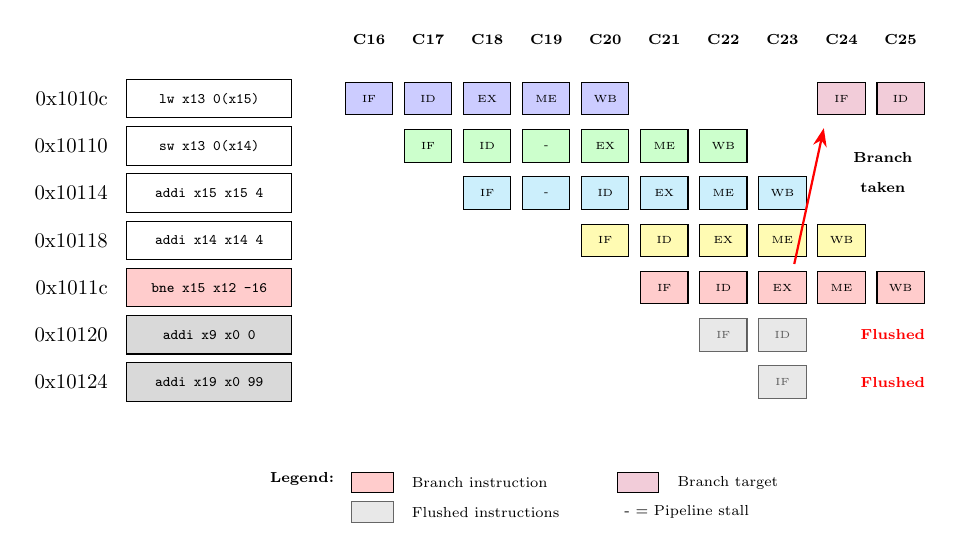
\begin{tikzpicture}[
    scale=0.75,
    transform shape,
    instruction/.style={rectangle, draw, minimum width=2.8cm, minimum height=0.65cm, font=\ttfamily\scriptsize},
    stage/.style={font=\scriptsize\bfseries},
    cycle/.style={font=\scriptsize\bfseries},
    arrow/.style={->, >=Stealth, thick, red}
]

% Cycle numbers at top
\foreach \i in {16,...,25} {
    \node[cycle] at (0.3 + 1.0*\i -15.0, 5.0) {C\i};
}

\node[ anchor=east] at (-3, 4.0) {0x1010c};
\node[ anchor=east] at (-3, 3.2) {0x10110};
\node[ anchor=east] at (-3, 2.4) {0x10114};
\node[ anchor=east] at (-3, 1.6) {0x10118};
\node[ anchor=east] at (-3, 0.8) {0x1011c};
\node[ anchor=east] at (-3, 0.0) {0x10120};
\node[ anchor=east] at (-3, -0.8) {0x10124};
% Instructions labels on the left

\node[instruction, anchor=east] at (0, 4.0) {lw x13 0(x15)};
\node[instruction, anchor=east] at (0, 3.2) {sw x13 0(x14)};
\node[instruction, anchor=east] at (0, 2.4) {addi x15 x15 4};
\node[instruction, anchor=east] at (0, 1.6) {addi x14 x14 4};
\node[instruction, anchor=east, fill=red!20] at (0, 0.8) {bne x15 x12 -16};
\node[instruction, anchor=east, fill=gray!30] at (0, 0.0) {addi x9 x0 0};
\node[instruction, anchor=east, fill=gray!30] at (0, -0.8) {addi x19 x0 99};

% lw x13 0 x15
\foreach \i/\stage in {1/IF, 2/ID, 3/EX, 4/ME, 5/WB, 9/IF, 10/ID} {
    \ifnum \i > 5
        \node[draw, fill=purple!20, minimum width=0.8cm, minimum height=0.55cm] at (0.3 + 1.0*\i, 4.0) {\tiny\stage};
    \else
        \node[draw, fill=blue!20, minimum width=0.8cm, minimum height=0.55cm] at (0.3 + 1.0*\i, 4.0) {\tiny\stage};
    \fi
}

% sw x13 0 x14
\foreach \i/\stage in {2/IF, 3/ID, 4/-, 5/EX, 6/ME, 7/WB} {
    \node[draw, fill=green!20, minimum width=0.8cm, minimum height=0.55cm] at (0.3 + 1.0*\i, 3.2) {\tiny\stage};
}

% addi x15 x15 4
\foreach \i/\stage in {3/IF, 4/-, 5/ID, 6/EX, 7/ME, 8/WB} {
    \node[draw, fill=cyan!20, minimum width=0.8cm, minimum height=0.55cm] at (0.3 + 1.0*\i, 2.4) {\tiny\stage};
}

% addi x14 x14 4 (shifted one cycle to the right)
\foreach \i/\stage in {5/IF, 6/ID, 7/EX, 8/ME, 9/WB} {
    \node[draw, fill=yellow!30, minimum width=0.8cm, minimum height=0.55cm] at (0.3 + 1.0*\i, 1.6) {\tiny\stage};
}

% bne x15 x12 -16 (branch taken) - shifted one cycle
\foreach \i/\stage in {6/IF, 7/ID, 8/EX, 9/ME, 10/WB} {
    \node[draw, fill=red!20, minimum width=0.8cm, minimum height=0.55cm] at (0.3 + 1.0*\i, 0.8) {\tiny\stage};
}

% addi x9 x0 0 (FLUSHED) - shifted one cycle
\foreach \i/\stage in {7/IF, 8/ID} {
    \node[draw, fill=gray!30, minimum width=0.8cm, minimum height=0.55cm, opacity=0.6] at (0.3 + 1.0*\i, 0.0) {\tiny\stage};
}
\node[font=\scriptsize\color{red}, anchor=west] at (9.5, 0.0) {\textbf{Flushed}};

% addi x19 x0 99 (FLUSHED) - shifted one cycle
\foreach \i/\stage in {8/IF} {
    \node[draw, fill=gray!30, minimum width=0.8cm, minimum height=0.55cm, opacity=0.6] at (0.3 + 1.0*\i, -0.8) {\tiny\stage};
}
\node[font=\scriptsize\color{red}, anchor=west] at (9.5, -0.8) {\textbf{Flushed}};


% Update the purple branch target stages


% Arrow showing branch resolution - adjusted position
\draw[arrow] (8.5, 1.2) -- (9, 3.5);
\node[font=\scriptsize] at (10, 3.0) {\textbf{Branch}};
\node[font=\scriptsize] at (10, 2.5) {\textbf{taken}};

% Legend
\node[font=\scriptsize\bfseries, anchor=north west] at (-0.5, -2.2) {\textbf{Legend:}};

\node[draw, fill=red!20, minimum width=0.7cm, minimum height=0.35cm, anchor=west] at (1.0, -2.5) {};
\node[font=\scriptsize, anchor=west] at (1.9, -2.5) {Branch instruction};

\node[draw, fill=gray!30, minimum width=0.7cm, minimum height=0.35cm, opacity=0.6, anchor=west] at (1.0, -3.0) {};
\node[font=\scriptsize, anchor=west] at (1.9, -3.0) {Flushed instructions};

\node[draw, fill=purple!20, minimum width=0.7cm, minimum height=0.35cm, anchor=west] at (5.5, -2.5) {};
\node[font=\scriptsize, anchor=west] at (6.4, -2.5) {Branch target};

\node[font=\scriptsize, anchor=west] at (5.5, -3.0) {- = Pipeline stall};

\end{tikzpicture}
\caption{Pipeline behavior showing instruction flushing when branch is taken.}
\label{fig:branch_flushing}
\end{figure}

The incomplete instructions occur due to \textbf{control hazards} caused by branch instructions. When a branch is taken, instructions that were speculatively fetched from the sequential path (fall-through) must be discarded. In the example shown, the two \texttt{addi} instructions (\texttt{addi x9 x0 0} and \texttt{addi x19 x0 99}) enter the pipeline after the branch instruction but before the branch outcome is determined. Once the branch is resolved as taken (in the EX stage), these instructions are flushed from the pipeline as they represent incorrect speculative execution. The processor must then begin fetching from the correct branch target address, which in this case returns to the \texttt{lw x13 0 x15} instruction, indicating a loop structure.

This flushing mechanism is necessary to maintain correct program semantics: executing instructions from the wrong path would produce incorrect results. The cost of this mechanism is the branch penalty—cycles wasted on instructions that do not contribute to program progress.

Additionally, the pipeline diagram reveals \textbf{pipeline stalls} (indicated by dashes "-" in the diagram), which occur due to \textbf{Data hazards} (data dependencies). For instance, the \texttt{sw x13 0 x14} instruction stalls in the ID stage because it depends on the result of the previous \texttt{lw} instruction, which hasn't yet completed its ME stage where the data is loaded.


\subsubsection{Branch Prediction Mechanism}
Based on the observed pipeline behavior of the first loop in \texttt{< main >} (Figure \ref{fig:branch_flushing_extended} ), the processor does \textbf{not appear to have a sophisticated branch predictor}.
The consistent pattern of pipeline flushing observed across all branch instructions indicates the absence of a dynamic branch predictor in this processor design. This conclusion is supported by several key observations:
\begin{itemize}
    \item \textbf{Consistent Flushing Pattern}: Every taken branch exhibits identical flushing behavior, regardless of execution history. This suggests a static approach rather than adaptive learning.

    \item \textbf{No Learning Observed}: In a typical dynamic branch predictor (such as a two-bit saturating counter or branch history table), we would expect:
    \begin{enumerate}
        \item \textbf{Initial iterations}: Flushes would occur as the predictor learns branch behavior
        \item \textbf{Subsequent iterations}: After 2 executions, the predictor would accurately predict the branch direction, eliminating flushes
    \end{enumerate}
    The insertion sort algorithm contains loop branches that are typically taken many times consecutively. A competent dynamic predictor would quickly learn this pattern and avoid flushing after the initial learning phase.

    \item \textbf{Statistical Evidence}: Analysis of the pipeline trace reveals that branches exhibit the same 2-cycle penalty (flushing 2 instructions) throughout execution, with no improvement over time. This static penalty pattern is characteristic of processors without branch prediction or with always-not-taken static prediction.
\end{itemize}

To illustrate what we would expect with a dynamic branch predictor, consider the following theoretical behavior pattern for a loop branch:

\begin{table}[H]
\centering
\vspace{0.3cm}
\renewcommand{\arraystretch}{1.4}
\scalebox{0.85}{ % Scale the entire table to 85% of original size
\begin{tabular}{|c|c|c|c|c|}
\hline
\rowcolor{blue!20}
\textbf{Branch Iteration} &
\textbf{Predicted Outcome} &
\textbf{Actual Outcome} &
\textbf{Pipeline Flush} &
\textbf{Predictor State Update} \\
\hline
\rowcolor{red!30}
1st & Strongly Not Taken (initial) & Taken & Yes (2 instructions) & Learn → Weakly Not Taken\\
\hline
\rowcolor{red!10}
2nd & Weakly Not Taken  & Taken & Yes (2 instructions) & Learn → Weakly Taken \\
\hline
\rowcolor{green!10}
3rd & Weakly Taken & Taken & No (correct prediction) & Learn → Strongly Taken \\
\hline
\rowcolor{green!30}
4th & Strongly Taken & Taken & No (correct prediction) & Maintain Strongly Taken \\
\hline
\rowcolor{green!30}
5th+ & Strongly Taken & Taken & No (correct prediction) & Maintain Strongly Taken \\
\hline
\end{tabular}
} % End of scalebox
\caption{Expected behavior of a two-bit saturating counter branch predictor}
\label{tab:branch_predictor_behavior}
\end{table}

Since our observations show \textbf{consistent flushing across all iterations}, we can conclude that no such learning mechanism exists in this implementation.
\begin{figure}[htbp]
\centering
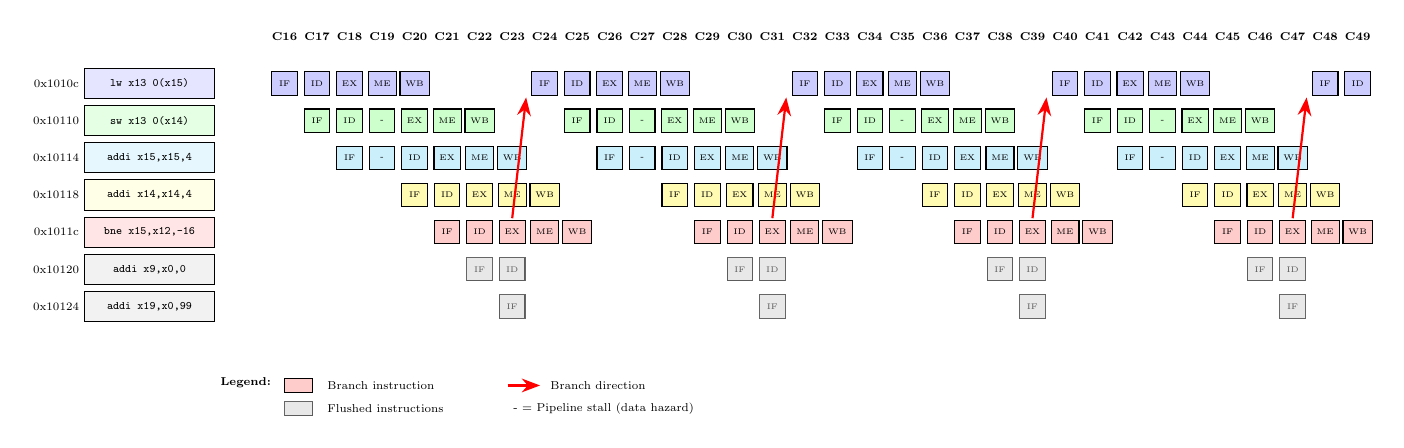
\begin{tikzpicture}[
    scale=0.59,
    transform shape,
    instruction/.style={rectangle, draw, minimum width=2.8cm, minimum height=0.65cm, font=\ttfamily\scriptsize},
    stage/.style={font=\scriptsize\bfseries},
    cycle/.style={font=\scriptsize\bfseries},
    arrow/.style={->, >= Stealth, thick, red}
]

% Cycle numbers at top - extended to show multiple iterations
\foreach \i in {16,...,49} {
    \node[cycle] at (4.8 + 0.7*\i-15, 5.0) {C\i};
}

% Program counter addresses
\node[anchor=east, font=\scriptsize] at (-3.3, 4.0) {0x1010c};
\node[anchor=east, font=\scriptsize] at (-3.3, 3.2) {0x10110};
\node[anchor=east, font=\scriptsize] at (-3.3, 2.4) {0x10114};
\node[anchor=east, font=\scriptsize] at (-3.3, 1.6) {0x10118};
\node[anchor=east, font=\scriptsize] at (-3.3, 0.8) {0x1011c};
\node[anchor=east, font=\scriptsize] at (-3.3, 0.0) {0x10120};
\node[anchor=east, font=\scriptsize] at (-3.3, -0.8) {0x10124};

% Instructions labels on the left
\node[instruction, anchor=east,fill=blue!10] at (-0.5, 4.0) {lw x13 0(x15)};
\node[instruction, anchor=east,fill=green!10] at (-0.5, 3.2) {sw x13 0(x14)};
\node[instruction, anchor=east,fill=cyan!10] at (-0.5, 2.4) {addi x15,x15,4};
\node[instruction, anchor=east,fill=yellow!10] at (-0.5, 1.6) {addi x14,x14,4};
\node[instruction, anchor=east, fill=red!10] at (-0.5, 0.8) {bne x15,x12,-16};
\node[instruction, anchor=east, fill=gray!10] at (-0.5, 0.0) {addi x9,x0,0};
\node[instruction, anchor=east, fill=gray!10] at (-0.5, -0.8) {addi x19,x0,99};

% First iteration: lw x13 0(x15)
\foreach \i/\stage in {1/IF, 2/ID, 3/EX, 4/ME, 5/WB} {
    \node[draw, fill=blue!20, minimum width=0.55cm, minimum height=0.5cm] at (0.3 + 0.7*\i, 4.0) {\tiny\stage};
}

% First iteration: sw x13 0(x14)
\foreach \i/\stage in {2/IF, 3/ID, 4/-, 5/EX, 6/ME, 7/WB} {
    \node[draw, fill=green!20, minimum width=0.55cm, minimum height=0.5cm] at (0.3 + 0.7*\i, 3.2) {\tiny\stage};
}

% First iteration: addi x15 x15 4
\foreach \i/\stage in {3/IF, 4/-, 5/ID, 6/EX, 7/ME, 8/WB} {
    \node[draw, fill=cyan!20, minimum width=0.55cm, minimum height=0.5cm] at (0.3 + 0.7*\i, 2.4) {\tiny\stage};
}

% First iteration: addi x14 x14 4
\foreach \i/\stage in {5/IF, 6/ID, 7/EX, 8/ME, 9/WB} {
    \node[draw, fill=yellow!30, minimum width=0.55cm, minimum height=0.5cm] at (0.3 + 0.7*\i, 1.6) {\tiny\stage};
}

% First iteration: bne (branch taken)
\foreach \i/\stage in {6/IF, 7/ID, 8/EX, 9/ME, 10/WB} {
    \node[draw, fill=red!20, minimum width=0.55cm, minimum height=0.5cm] at (0.3 + 0.7*\i, 0.8) {\tiny\stage};
}

% First iteration: addi x9 (FLUSHED)
\foreach \i/\stage in {7/IF, 8/ID} {
    \node[draw, fill=gray!30, minimum width=0.55cm, minimum height=0.5cm, opacity=0.6] at (0.3 + 0.7*\i, 0.0) {\tiny\stage};
}

% First iteration: addi x19 (FLUSHED)
\foreach \i/\stage in {8/IF} {
    \node[draw, fill=gray!30, minimum width=0.55cm, minimum height=0.5cm, opacity=0.6] at (0.3 + 0.7*\i, -0.8) {\tiny\stage};
}

% Second iteration: lw x13 0(x15)
\foreach \i/\stage in {9/IF, 10/ID, 11/EX, 12/ME, 13/WB} {
    \node[draw, fill=blue!20, minimum width=0.55cm, minimum height=0.5cm] at (0.3 + 0.7*\i, 4.0) {\tiny\stage};
}

% Second iteration: sw x13 0(x14)
\foreach \i/\stage in {10/IF, 11/ID, 12/-, 13/EX, 14/ME, 15/WB} {
    \node[draw, fill=green!20, minimum width=0.55cm, minimum height=0.5cm] at (0.3 + 0.7*\i, 3.2) {\tiny\stage};
}

% Second iteration: addi x15 x15 4
\foreach \i/\stage in {11/IF, 12/-, 13/ID, 14/EX, 15/ME, 16/WB} {
    \node[draw, fill=cyan!20, minimum width=0.55cm, minimum height=0.5cm] at (0.3 + 0.7*\i, 2.4) {\tiny\stage};
}

% Second iteration: addi x14 x14 4
\foreach \i/\stage in {13/IF, 14/ID, 15/EX, 16/ME, 17/WB} {
    \node[draw, fill=yellow!30, minimum width=0.55cm, minimum height=0.5cm] at (0.3 + 0.7*\i, 1.6) {\tiny\stage};
}

% Second iteration: bne (branch taken)
\foreach \i/\stage in {14/IF, 15/ID, 16/EX, 17/ME, 18/WB} {
    \node[draw, fill=red!20, minimum width=0.55cm, minimum height=0.5cm] at (0.3 + 0.7*\i, 0.8) {\tiny\stage};
}

% Second iteration: addi x9 (FLUSHED)
\foreach \i/\stage in {15/IF, 16/ID} {
    \node[draw, fill=gray!30, minimum width=0.55cm, minimum height=0.5cm, opacity=0.6] at (0.3 + 0.7*\i, 0.0) {\tiny\stage};
}

% Second iteration: addi x19 (FLUSHED)
\foreach \i/\stage in {16/IF} {
    \node[draw, fill=gray!30, minimum width=0.55cm, minimum height=0.5cm, opacity=0.6] at (0.3 + 0.7*\i, -0.8) {\tiny\stage};
}

% Third iteration: lw x13 0(x15)
\foreach \i/\stage in {17/IF, 18/ID, 19/EX, 20/ME, 21/WB} {
    \node[draw, fill=blue!20, minimum width=0.55cm, minimum height=0.5cm] at (0.3 + 0.7*\i, 4.0) {\tiny\stage};
}

% Third iteration: sw x13 0(x14)
\foreach \i/\stage in {18/IF, 19/ID, 20/-, 21/EX, 22/ME, 23/WB} {
    \node[draw, fill=green!20, minimum width=0.55cm, minimum height=0.5cm] at (0.3 + 0.7*\i, 3.2) {\tiny\stage};
}

% Third iteration: addi x15 x15 4
\foreach \i/\stage in {19/IF, 20/-, 21/ID, 22/EX, 23/ME, 24/WB} {
    \node[draw, fill=cyan!20, minimum width=0.55cm, minimum height=0.5cm] at (0.3 + 0.7*\i, 2.4) {\tiny\stage};
}

% Third iteration: addi x14 x14 4
\foreach \i/\stage in {21/IF, 22/ID, 23/EX, 24/ME, 25/WB} {
    \node[draw, fill=yellow!30, minimum width=0.55cm, minimum height=0.5cm] at (0.3 + 0.7*\i, 1.6) {\tiny\stage};
}

% Third iteration: bne (branch taken)
\foreach \i/\stage in {22/IF, 23/ID, 24/EX, 25/ME, 26/WB} {
    \node[draw, fill=red!20, minimum width=0.55cm, minimum height=0.5cm] at (0.3 + 0.7*\i, 0.8) {\tiny\stage};
}

% Third iteration: addi x9 (FLUSHED)
\foreach \i/\stage in {23/IF, 24/ID} {
    \node[draw, fill=gray!30, minimum width=0.55cm, minimum height=0.5cm, opacity=0.6] at (0.3 + 0.7*\i, 0.0) {\tiny\stage};
}

% Third iteration: addi x19 (FLUSHED)
\foreach \i/\stage in {24/IF} {
    \node[draw, fill=gray!30, minimum width=0.55cm, minimum height=0.5cm, opacity=0.6] at (0.3 + 0.7*\i, -0.8) {\tiny\stage};
}

% Fourth iteration: lw x13 0(x15)
\foreach \i/\stage in {25/IF, 26/ID, 27/EX, 28/ME, 29/WB} {
    \node[draw, fill=blue!20, minimum width=0.55cm, minimum height=0.5cm] at (0.3 + 0.7*\i, 4.0) {\tiny\stage};
}

% Fourth iteration: sw x13 0(x14)
\foreach \i/\stage in {26/IF, 27/ID, 28/-, 29/EX, 30/ME, 31/WB} {
    \node[draw, fill=green!20, minimum width=0.55cm, minimum height=0.5cm] at (0.3 + 0.7*\i, 3.2) {\tiny\stage};
}

% Fourth iteration: addi x15 x15 4
\foreach \i/\stage in {27/IF, 28/-, 29/ID, 30/EX, 31/ME, 32/WB} {
    \node[draw, fill=cyan!20, minimum width=0.55cm, minimum height=0.5cm] at (0.3 + 0.7*\i, 2.4) {\tiny\stage};
}

% Fourth iteration: addi x14 x14 4
\foreach \i/\stage in {29/IF, 30/ID, 31/EX, 32/ME, 33/WB} {
    \node[draw, fill=yellow!30, minimum width=0.55cm, minimum height=0.5cm] at (0.3 + 0.7*\i, 1.6) {\tiny\stage};
}

% Fourth iteration: bne (branch taken)
\foreach \i/\stage in {30/IF, 31/ID, 32/EX, 33/ME, 34/WB} {
    \node[draw, fill=red!20, minimum width=0.55cm, minimum height=0.5cm] at (0.3 + 0.7*\i, 0.8) {\tiny\stage};
}

% Fourth iteration: addi x9 (FLUSHED)
\foreach \i/\stage in {31/IF, 32/ID} {
    \node[draw, fill=gray!30, minimum width=0.55cm, minimum height=0.5cm, opacity=0.6] at (0.3 + 0.7*\i, 0.0) {\tiny\stage};
}

% Fourth iteration: addi x19 (FLUSHED)
\foreach \i/\stage in {32/IF} {
    \node[draw, fill=gray!30, minimum width=0.55cm, minimum height=0.5cm, opacity=0.6] at (0.3 + 0.7*\i, -0.8) {\tiny\stage};
}

% Fifth iteration start: lw x13 0(x15)
\foreach \i/\stage in {33/IF, 34/ID} {
    \node[draw, fill=blue!20, minimum width=0.55cm, minimum height=0.5cm] at (0.3 + 0.7*\i, 4.0) {\tiny\stage};
}

% Arrows showing branch resolution points
\draw[arrow] (5.9, 1.1) -- (6.2, 3.7);
\draw[arrow] (11.5, 1.1) -- (11.8, 3.7);
\draw[arrow] (17.1, 1.1) -- (17.4, 3.7);
\draw[arrow] (22.7, 1.1) -- (23, 3.7);

% Legend
\node[font=\scriptsize\bfseries, anchor=north west] at (-0.5, -2.2) {\textbf{Legend:}};

\node[draw, fill=red!20, minimum width=0.6cm, minimum height=0.3cm, anchor=west] at (1.0, -2.5) {};
\node[font=\scriptsize, anchor=west] at (1.8, -2.5) {Branch instruction};

\node[draw, fill=gray!30, minimum width=0.6cm, minimum height=0.3cm, opacity=0.6, anchor=west] at (1.0, -3.0) {};
\node[font=\scriptsize, anchor=west] at (1.8, -3.0) {Flushed instructions};

\node[font=\scriptsize, anchor=north west] at (6.6, -2.3) {Branch direction};
\draw[arrow] (5.8, -2.5) -- (6.5, -2.5);
\node[font=\scriptsize, anchor=west] at (5.8, -3.0) {- = Pipeline stall (data hazard)};

\end{tikzpicture}
\caption{Pipeline diagram showing multiple loop iterations with repeated branch taken behavior and instruction flushing.}
\label{fig:branch_flushing_extended}
\end{figure}


\subsubsection{Optimal CPI}
The optimal Cycles Per Instruction (CPI) for a simple 5-stage scalar pipelined processor is \textbf{1.0}. In an ideal scenario without hazards, each stage of the pipeline is fully utilized, and the processor can complete and retire a new instruction on every clock cycle. This is achieved by overlapping the execution of instructions across the five stages (IF, ID, EX, ME, WB).

\subsubsection{Analysis of Observed Performance}
The simulation of the insertion sort program yielded an observed CPI of \textbf{1.38}. This significant deviation from the optimal value of 1.0 indicates that pipeline hazards cause the processor to stall or flush for approximately 38\% of the total cycles. The performance penalty can be attributed to the two primary types of pipeline hazards present in the code.

\begin{itemize}
    \item \textbf{Control Hazards (Branch Penalties):} Branches and jumps are resolved in the Execute (EX) stage. When a branch is taken, the instructions already fetched into the pipeline based on the incorrect program path (the next sequential addresses) must be discarded. As specified in the lecture, this results in a two-cycle penalty to flush the pipeline, making the effective cost of a taken branch three cycles. The insertion sort algorithm is dominated by tight loops, leading to frequent taken branches that incur this penalty and elevate the average CPI.

    \item \textbf{Data Hazards (Load-Use Stalls):} A critical data hazard occurs when an instruction immediately uses a value loaded from memory. A load instruction (\texttt{lw}) produces its result at the end of the Memory (ME) stage. If the very next instruction requires that value as an input for its Execute stage, a one-cycle stall (or bubble) must be inserted into the pipeline. Even with forwarding hardware, the data from a load is not available in time for the next instruction's EX stage, necessitating this delay.
\end{itemize}

\noindent
\begin{minipage}{\linewidth}
The following code segment from the insertion sort inner loop clearly illustrates both hazards in action:
% In the document body:
\begin{lstlisting}[style=mystyle]
1010c:  0007a683  lw  x13, 0(x15)  ; Load from memory
10110:  00d72023  sw  x13, 0(x14)  ; *Data Hazard: Uses x13 immediately*
10114:  00478793  addi x15, x15, 4
10118:  00470713  addi x14, x14, 4
1011c:  fec798e3  bne  x15, x12, -16 ; *Control Hazard: Frequent taken branch*
\end{lstlisting}
\end{minipage}

At address \texttt{1010c}, the \texttt{lw} instruction creates a load-use hazard with the subsequent \texttt{sw} at \texttt{10110}, requiring a stall. Later, the \texttt{bne} instruction at \texttt{1011c} is a backward branch that ends the loop iteration. When taken, it flushes the incorrectly fetched sequential instructions, incurring the branch penalty. The frequent execution of this loop structure makes these hazards the dominant cause of the elevated CPI.



\subsubsection{Comparison with Lecture Analysis}

The lecture provides a theoretical analysis of processor performance based on a typical instruction mix. The theoretical average CPI derived in the lecture is \textbf{1.47}. This calculation assumes:

\begin{itemize}
    \item 11\% of instructions are loads that cause stalls (2 cycles).
    \item 18\% of instructions are control flow (jumps or taken branches) incurring heavy penalties (3 cycles).
    \item A base CPI of 1.0 for arithmetic and other instructions .
\end{itemize}

The observed CPI for the insertion sort program (\textbf{1.38}) is slightly better (lower) than the lecture's theoretical average (\textbf{1.47}).
This discrepancy suggests that the specific instruction mix of the  insertion sort  is more efficient than the generic benchmark assumed in the lecture. Specifically, the insertion sort implementation likely contains a higher proportion of "safe" arithmetic/logic instructions relative to expensive control flow or load-use hazards, or the specific arrangement of instructions allows for fewer data stalls than the 11\% assumed in the general model.

\subsection{6-stage dual issue processor}
To understand the performance characteristics of the dual-issue configuration, we must first examine its underlying architecture. The simulated processor extends the classic pipeline into a 6-stage, dual-issue in-order design, as visually represented in the architectural diagram from the \textbf{Ripes} simulator shown in Figure~\ref{fig:6stage_dual_issue_pipeline}. This enhanced design aims to improve throughput by fetching, decoding, and executing two instructions per cycle.
\begin{figure}[h]
    \centering
    \includegraphics[width=0.9\linewidth]{img/6-stage_RISC-V_processor.jpeg}
    \caption{Diagram of the 6-stage dual issue RISC-V pipeline architecture }
    \label{fig:6stage_dual_issue_pipeline}
\end{figure}


The enhanced pipeline consists of the following stages:
\begin{enumerate}
    \item \textbf{Instruction Fetch (IF):} Retrieve up to two instructions per cycle from memory.
    \item \textbf{Instruction Decode (ID):} Decode both instructions and read register values.
    \item \textbf{Instruction Issue (II):} Determine if both instructions can be issued simultaneously based on dependencies.
    \item \textbf{Execute (EX):} Perform arithmetic/logic operations in parallel execution units.
    \item \textbf{Memory Access (ME):} Access data memory for load/store operations.
    \item \textbf{Write Back (WB):} Write results back to the register file through multiple write ports.
\end{enumerate}

This design aims to achieve a theoretical throughput of two instructions per cycle (CPI = 0.5). However, practical limitations including dependencies, resource conflicts, and hazards reduce this ideal performance, as observed in the following analysis.


\subsubsection{Pipeline Behavior Analysis}

Figure~\ref{fig:dual_issue_hazards} illustrates the detailed timing behavior of the pipeline during execution of the array copy loop. The diagram clearly shows that although two instructions are frequently fetched together, they are not consistently able to progress through all stages simultaneously.



\begin{figure}[htbp]
\centering
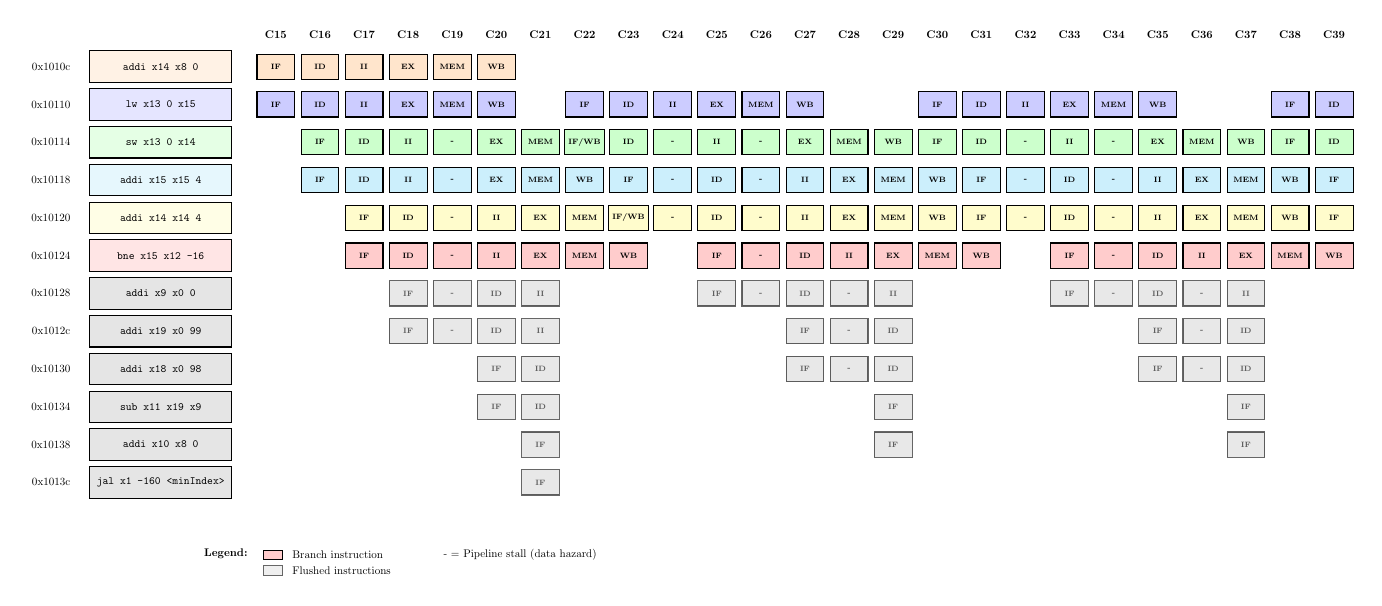
\begin{tikzpicture}[
    scale=0.4, % Ajuste l'échelle globale pour que le grand diagramme tienne sur la page
    transform shape,
    instruction/.style={rectangle, draw, minimum width=4.5cm, minimum height=1cm, font=\ttfamily\normalsize, anchor=east},
    stage/.style={draw, minimum width=1.2cm, minimum height=0.8cm, font=\scriptsize\bfseries},
    stall/.style={draw, fill=gray!20, minimum width=1.4cm, minimum height=1cm, font=\scriptsize\bfseries},
    header/.style={font=\normalsize\bfseries}
]


\foreach \i in {15,...,39} {
    \node[header] at (-1.4*14+1.4*\i, 1) {C\i};
}
% Program counter addresses
\node[anchor=east, font=\normalsize] at (-5, 0) {0x1010c};
\node[anchor=east, font=\normalsize] at (-5, -1*1.2) {0x10110};
\node[anchor=east, font=\normalsize] at (-5, -2*1.2) {0x10114};
\node[anchor=east, font=\normalsize] at (-5, -3*1.2) {0x10118};
\node[anchor=east, font=\normalsize] at (-5, -4*1.2) {0x10120};
\node[anchor=east, font=\normalsize] at (-5, -5*1.2) {0x10124};
\node[anchor=east, font=\normalsize] at (-5, -6*1.2) {0x10128};
\node[anchor=east, font=\normalsize] at (-5, -7*1.2) {0x1012c};
\node[anchor=east, font=\normalsize] at (-5, -8*1.2) {0x10130};
\node[anchor=east, font=\normalsize] at (-5, -9*1.2) {0x10134};
\node[anchor=east, font=\normalsize] at (-5, -10*1.2) {0x10138};
\node[anchor=east, font=\normalsize] at (-5, -11*1.2) {0x1013c};
% --- Libellés des Instructions ---
\node[instruction,fill=orange!10] at (0, 0) {addi x14 x8 0};
\node[instruction,fill=blue!10] at (0, -1*1.2) {lw x13 0 x15};
\node[instruction,fill=green!10] at (0, -2*1.2) {sw x13 0 x14};
\node[instruction,fill=cyan!10] at (0, -3*1.2) {addi x15 x15 4};
\node[instruction,fill=yellow!10] at (0, -4*1.2) {addi x14 x14 4};
\node[instruction,fill=red!10] at (0, -5*1.2) {bne x15 x12 -16};
\node[instruction, fill=gray!20] at (0, -6*1.2) {addi x9 x0 0};
\node[instruction, fill=gray!20] at (0, -7*1.2) {addi x19 x0 99};
\node[instruction, fill=gray!20] at (0, -8*1.2) {addi x18 x0 98};
\node[instruction, fill=gray!20] at (0, -9*1.2) {sub x11 x19 x9};
\node[instruction, fill=gray!20] at (0, -10*1.2) {addi x10 x8 0};
\node[instruction, fill=gray!20] at (0, -11*1.2) {jal x1 -160 <minIndex>};



% addi x14 x8 0
\foreach \c/\s in {1/IF, 2/ID, 3/II, 4/EX, 5/MEM, 6/WB} \node[stage, fill=orange!20] at (1.4*\c, 0) {\s};

% lw x13 0 x15
\foreach \c/\s in {1/IF, 2/ID, 3/II, 4/EX, 5/MEM, 6/WB, 8/IF, 9/ID, 10/II, 11/EX, 12/MEM, 13/WB, 16/IF, 17/ID, 18/II, 19/EX, 20/MEM, 21/WB , 24/IF ,25/ID}
    \node[stage, fill=blue!20] at (1.4*\c, -1*1.2) {\s};

% sw x13 0 x14
\foreach \c/\s in {2/IF, 3/ID, 4/II, 5/-, 6/EX, 7/MEM, 8/{IF/WB}, 9/ID, 10/-, 11/II, 12/-, 13/EX, 14/MEM, 15/WB, 16/IF, 17/ID, 18/-, 19/II, 20/-, 21/EX,22/MEM , 23/WB ,23/WB ,24/IF ,25/ID}
    \node[stage, fill=green!20] at (1.4*\c, -2*1.2) {\s};

% addi x15 x15 4
\foreach \c/\s in {2/IF, 3/ID, 4/II, 5/-, 6/EX, 7/MEM, 8/WB, 9/IF, 10/-, 11/ID, 12/-, 13/II, 14/EX, 15/MEM, 16/WB, 17/IF, 18/-, 19/ID, 20/-, 21/II, 22/EX , 23/MEM ,24/WB ,25/IF}
    \node[stage, fill=cyan!20] at (1.4*\c, -3*1.2) {\s};

% addi x14 x14 4
\foreach \c/\s in {3/IF, 4/ID, 5/-, 6/II, 7/EX, 8/MEM, 9/{IF/WB}, 10/-, 11/ID, 12/-, 13/II, 14/EX, 15/MEM, 16/WB, 17/IF, 18/-, 19/ID, 20/-, 21/II, 22/EX , 23/MEM ,24/WB ,25/IF}
    \node[stage, fill=yellow!20] at (1.4*\c, -4*1.2) {\s};

% bne x15 x12 -16
\foreach \c/\s in {3/IF, 4/ID, 5/-, 6/II, 7/EX, 8/MEM, 9/WB, 11/IF, 12/-, 13/ID, 14/II, 15/EX, 16/MEM, 17/WB, 19/IF, 20/-, 21/ID, 22/II, 23/EX, 24/MEM, 25/WB}
    \node[stage, fill=red!20] at (1.4*\c, -5*1.2) {\s};

% --- Instructions Flushed (Grisées) ---
% addi x9
\foreach \c/\s in {4/IF, 5/-, 6/ID, 7/II, 11/IF, 12/-, 13/ID, 14/-, 15/II, 19/IF, 20/-, 21/ID, 22/-, 23/II}
    \node[stage, fill=gray!30 ,opacity=0.6] at (1.4*\c, -6*1.2) {\s};

% addi x19
\foreach \c/\s in {4/IF, 5/-, 6/ID, 7/II, 13/IF, 14/-, 15/ID, 21/IF, 22/-, 23/ID}
    \node[stage, fill=gray!30 ,opacity=0.6] at (1.4*\c, -7*1.2) {\s};

% addi x18
\foreach \c/\s in {6/IF, 7/ID, 13/IF, 14/-, 15/ID, 21/IF, 22/-, 23/ID}
    \node[stage,fill=gray!30 ,opacity=0.6] at (1.4*\c, -8*1.2) {\s};

% sub x11
\foreach \c/\s in {6/IF, 7/ID, 15/IF, 23/IF}
    \node[stage, fill=gray!30 ,opacity=0.6] at (1.4*\c, -9*1.2) {\s};

% addi x10
\foreach \c/\s in {7/IF, 15/IF, 23/IF}
    \node[stage, fill=gray!30 ,opacity=0.6] at (1.4*\c, -10*1.2) {\s};

% jal x1
\node[stage, fill=gray!30 ,opacity=0.6] at (1.4*7, -11*1.2) {IF};


% Legend
\node[font=\normalsize\bfseries, anchor=north west] at (-1, -2.2-13) {\textbf{Legend:}};

\node[draw, fill=red!20, minimum width=0.6cm, minimum height=0.3cm, anchor=west] at (1.0, -2.5-13) {};
\node[font=\normalsize, anchor=west] at (1.8, -2.5-13) {Branch instruction};

\node[draw, fill=gray!20, minimum width=0.6cm, minimum height=0.3cm, opacity=0.6, anchor=west] at (1.0, -3.0-13) {};
\node[font=\normalsize, anchor=west] at (1.8, -3.0-13) {Flushed instructions};

\node[font=\normalsize, anchor=west] at (6.6, -2.5-13)  {- = Pipeline stall (data hazard)};



\end{tikzpicture}
\caption{Pipeline behavior during the array copy loop.}
\label{fig:dual_issue_hazards}
\end{figure}
A dominant factor limiting parallelism is the presence of data dependencies (RAW hazards). For instance, the instruction:

\begin{lstlisting}[style=mystyle]
lw x13, 0(x15)
\end{lstlisting}

produces a value that is immediately consumed by:

\begin{lstlisting}[style=mystyle]
sw x13, 0(x14)
\end{lstlisting}

Since the store instruction depends on the result of the load, it cannot proceed to execution before the load completes its memory stage. Even with forwarding mechanisms, load-use latency introduces unavoidable stalls. This creates visible bubbles in the pipeline and prevents effective dual issue.

Furthermore, pointer update instructions such as:

\begin{lstlisting}[style=mystyle]
addi x15, x15, 4
addi x14, x14, 4
\end{lstlisting}

are directly followed by the branch instruction:

\begin{lstlisting}[style=mystyle]
bne x15, x12, -16
\end{lstlisting}

The branch depends on the updated value of \texttt{x15}. Since branch resolution occurs only after the execute stage, the processor cannot immediately determine the next program counter value. As shown in the diagram, incorrectly fetched instructions are flushed when the branch is taken, leading to additional wasted cycles. These control hazards significantly reduce overall efficiency.

Another key observation from the diagram is that many cycles utilize only one execution slot despite the dual-issue capability. Because the processor operates in-order, an instruction that cannot be issued blocks subsequent instructions, even if they are independent. This strict ordering severely limits the exploitation of Instruction-Level Parallelism (ILP).

Overall, the pipeline behavior demonstrates that the dual-issue capability is frequently underutilized due to dependency chains and control hazards.
\subsubsection{Instruction Pairing and Issue Constraints}

Efficient instruction pairing in a dual-issue in-order processor requires the presence of independent instructions in close proximity. However, the array copy loop exhibits a strongly sequential structure. Most instructions either produce values immediately consumed by the next instruction or modify loop control variables used shortly afterward.

The issue stage performs conservative dependency checks and only allows two instructions to proceed simultaneously if no data hazards are detected and if execution resources are available. In this workload, long dependency chains effectively serialize execution.

Although the dual-issue architecture includes multiple register read and write ports to support parallel decode and write-back operations, the instruction stream rarely provides sufficient independent work to exploit these resources efficiently. Thus, the hardware capability exceeds the parallelism exposed by the program.

\subsubsection{Performance Analysis}

The measured CPI of \textbf{1.26} represents an improvement compared to the 5-stage single-issue processor, which achieved a CPI of 1.38. This corresponds to an approximate 8.7\% performance gain. While this confirms that additional parallelism is being exploited, the improvement remains far from the theoretical optimum of 0.5 CPI.

The primary limitation arises from the inherently sequential nature of the algorithm. Insertion sort contains tight dependency chains, particularly within inner loops, which restrict the availability of independent instructions. As a result, the second issue slot frequently remains unused.

Control hazards further degrade performance. The loop contains frequent branch instructions whose outcomes depend on recently computed values. Without advanced branch prediction or speculative execution mechanisms, each misprediction introduces pipeline flushing and wasted cycles.

Microarchitectural constraints also contribute to the performance gap. Since the processor executes instructions strictly in program order, it cannot dynamically reorder independent instructions to fill unused issue slots. More advanced superscalar processors employ out-of-order execution, register renaming, and dynamic scheduling to overcome this limitation. In contrast, this simpler dual-issue design can only exploit ILP that naturally appears in program order.

Finally, the instruction mix plays a significant role. A considerable portion of instructions are memory operations, making the workload partially memory-bound. In such cases, increasing ALU resources does not proportionally improve performance because memory latency becomes the dominant bottleneck.


\subsubsection{Optimal CPI}

The theoretical optimal CPI of 0.5 assumes that two independent instructions are always available, that sufficient functional units exist, and that no hazards or stalls occur. Achieving this level of performance requires abundant ILP, perfect branch prediction, and balanced resource availability.

In practice, these conditions are not satisfied. The workload exposes limited parallelism, branch behavior introduces control penalties, and structural constraints restrict simultaneous execution of certain instruction classes. Consequently, the observed CPI of 1.26 reflects a realistic balance between architectural capability and workload characteristics.

This analysis highlights an important architectural insight: increasing issue width does not automatically guarantee proportional performance improvement. The effectiveness of dual-issue execution depends strongly on the inherent parallelism of the workload and the sophistication of the microarchitectural mechanisms used to exploit it.

\subsubsection{Comparison with 5-Stage Processor}
Table~\ref{tab:processor_comparison} presents a comparison between the classical 5-stage pipeline and the 6-stage dual-issue architecture. Although the dual-issue processor offers a theoretical CPI of 0.5 compared to 1.0 for the single-issue design, this ideal 2× speedup is not achieved in practice.

The measured CPI decreases from 1.38 to 1.26, corresponding to an improvement of about 9\%. Similarly,indicating that the second issue slot is utilized in some cycles but remains frequently underused. This confirms that the workload exposes limited Instruction-Level Parallelism (ILP), preventing full exploitation of the dual-issue capability.
It is also important to note that the branch penalty increases from 2 cycles to 3 cycles due to the deeper pipeline. As a result, control hazards become slightly more expensive, partially offsetting the throughput gains provided by dual issue.


\begin{table}[H]
\centering
\renewcommand{\arraystretch}{1.4}
\begin{tabular}{|p{0.2\textwidth}|p{0.2\textwidth}|p{0.2\textwidth}|p{0.2\textwidth}|}
\hline
\rowcolor{blue!20}
\textbf{Metric} & \textbf{5-Stage} & \textbf{6-Stage Dual-Issue} & \textbf{Improvement} \\
\hline
Theoretical CPI & 1.0 & 0.5 & 2.0× \\
Achieved CPI & 1.38 & 1.26 & 1.09× \\
Branch Penalty & 2 cycles & 3 cycles & Worse \\
\hline
\end{tabular}
\caption{Performance comparison between processor configurations}
\label{tab:processor_comparison}
\end{table}



\end{document}


%%%%%%%%%%%%%%%%%%%%%%%%%%%%%%%%%%%%%%%%%%%%%%%%%%%%%%%%%%%%%%%%%


% SECTION BIBLIOGRAPHY

%%%%%%%%%%%%%%%%%%%%%%%%%%%%%%%%%%%%%%%%%%%%%%%%%%%%%%%%%%%%%%%%

\newpage % keep bibliography on a new page
\bibliographystyle{plain}   % choose a style
\bibliography{ref}      % name of .bib file (no .bib extension)


\end{document}
